\section{Exploratory Data Analysis}
\label{sec:eda}

The exploratory analysis pursues four questions in order. What does
the target variable look like over time and in distribution? Where are
the data missing, and what was done about it? Which anomalies stand
out? And which feature pairs are most strongly correlated, in
particular outside the rate corridor? The implementation lives in
\texttt{stage2\_alignment\_db.py} and \texttt{stage3\_advanced\_eda.py}.

\subsection{Target variable: WACMR}

Figure~\ref{fig:target-timeseries} plots the entire weekly WACMR
series. The visual pattern is striking: a slow downtrend through the
2014--2019 period, a sharp drop in March 2020, an extended low-rate
plateau through late 2021, and a re-tightening cycle that begins in
mid-2022 and is still incomplete at the end of the window. The
distribution in Figure~\ref{fig:eda-distributions} is visibly bimodal,
with one mode near 4.8\% (post-COVID accommodation) and another near
6.6\% (the pre-COVID normal). Bimodality of this kind is itself a
signal of regime non-stationarity, and motivates the unsupervised
clustering analysis in Section~\ref{sec:methods}.

\begin{figure}[H]
\centering
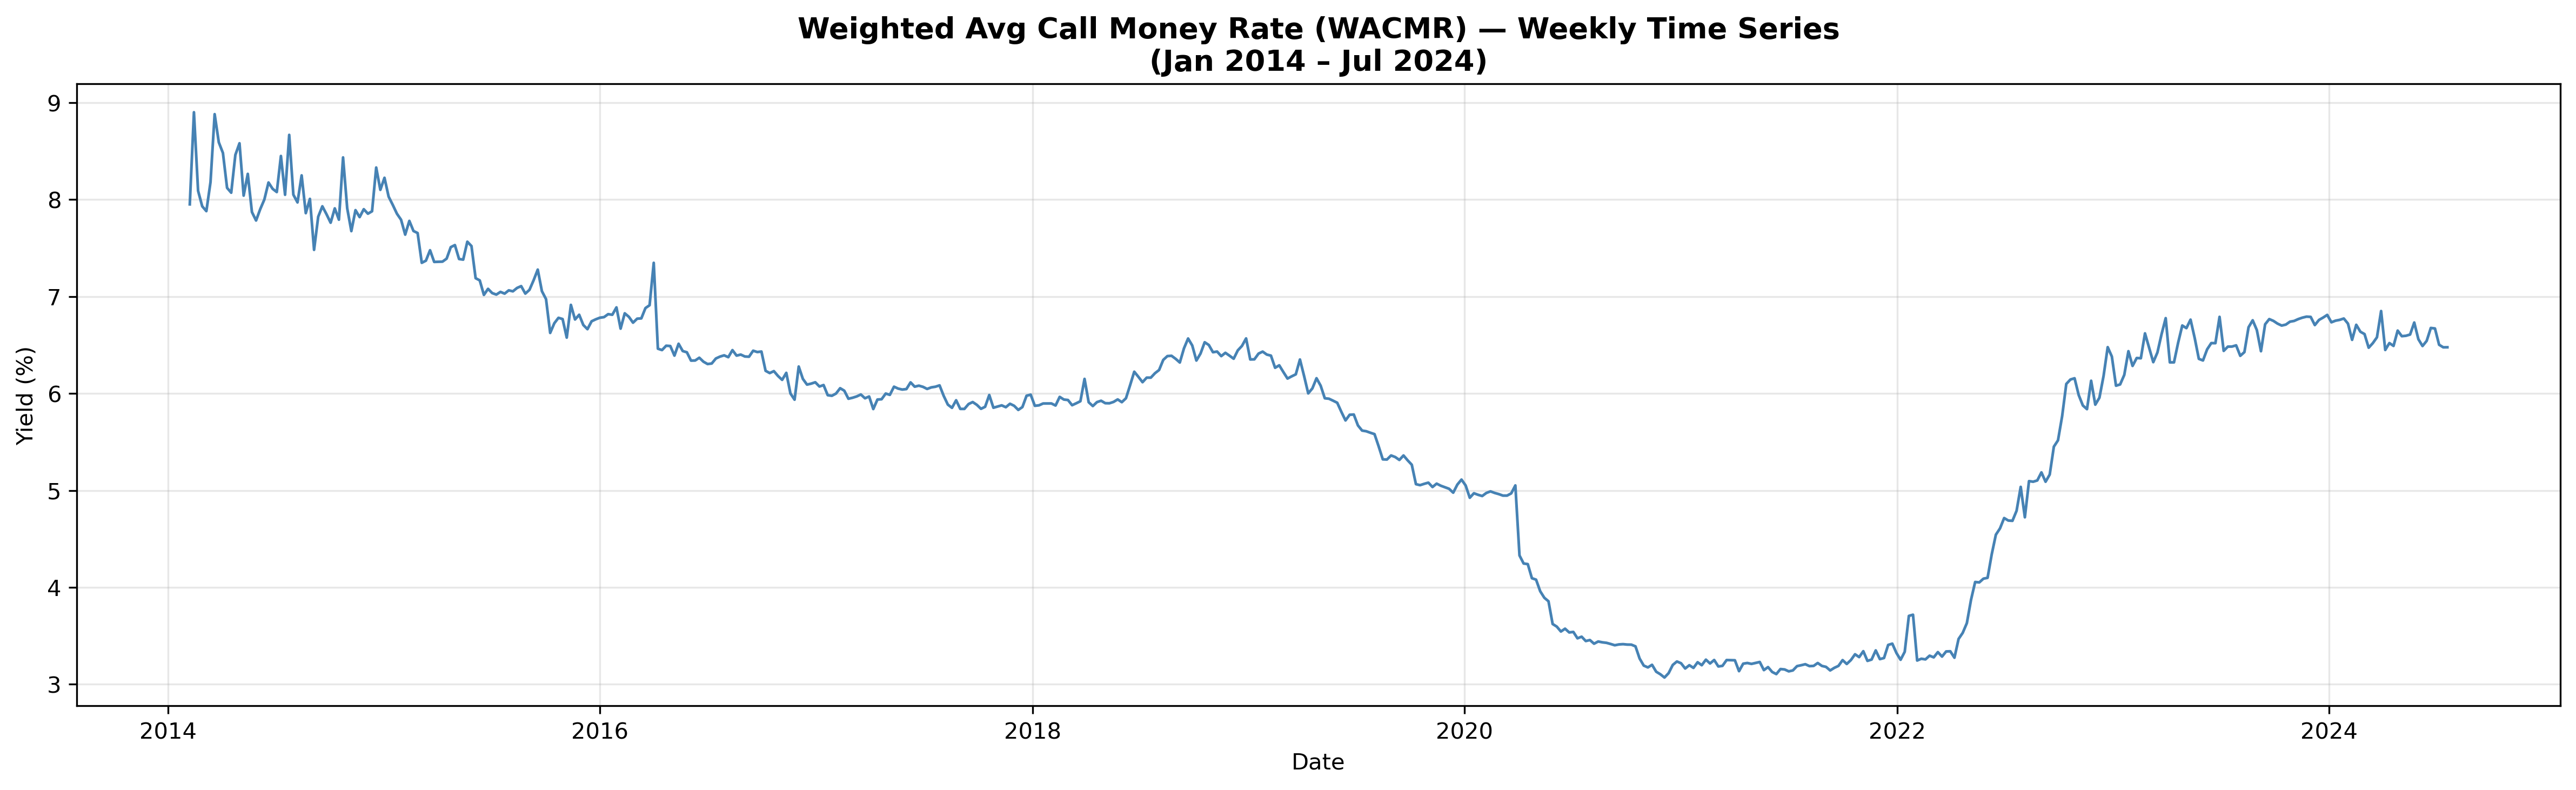
\includegraphics[width=0.92\linewidth]{../../visualizations/target_timeseries.png}
\caption{Weekly WACMR series, February 2014 to July 2024. The post-2020
drop is visually unmistakable and is the primary motivator for the
regime-clustering analysis.}
\label{fig:target-timeseries}
\end{figure}

\begin{figure}[H]
\centering
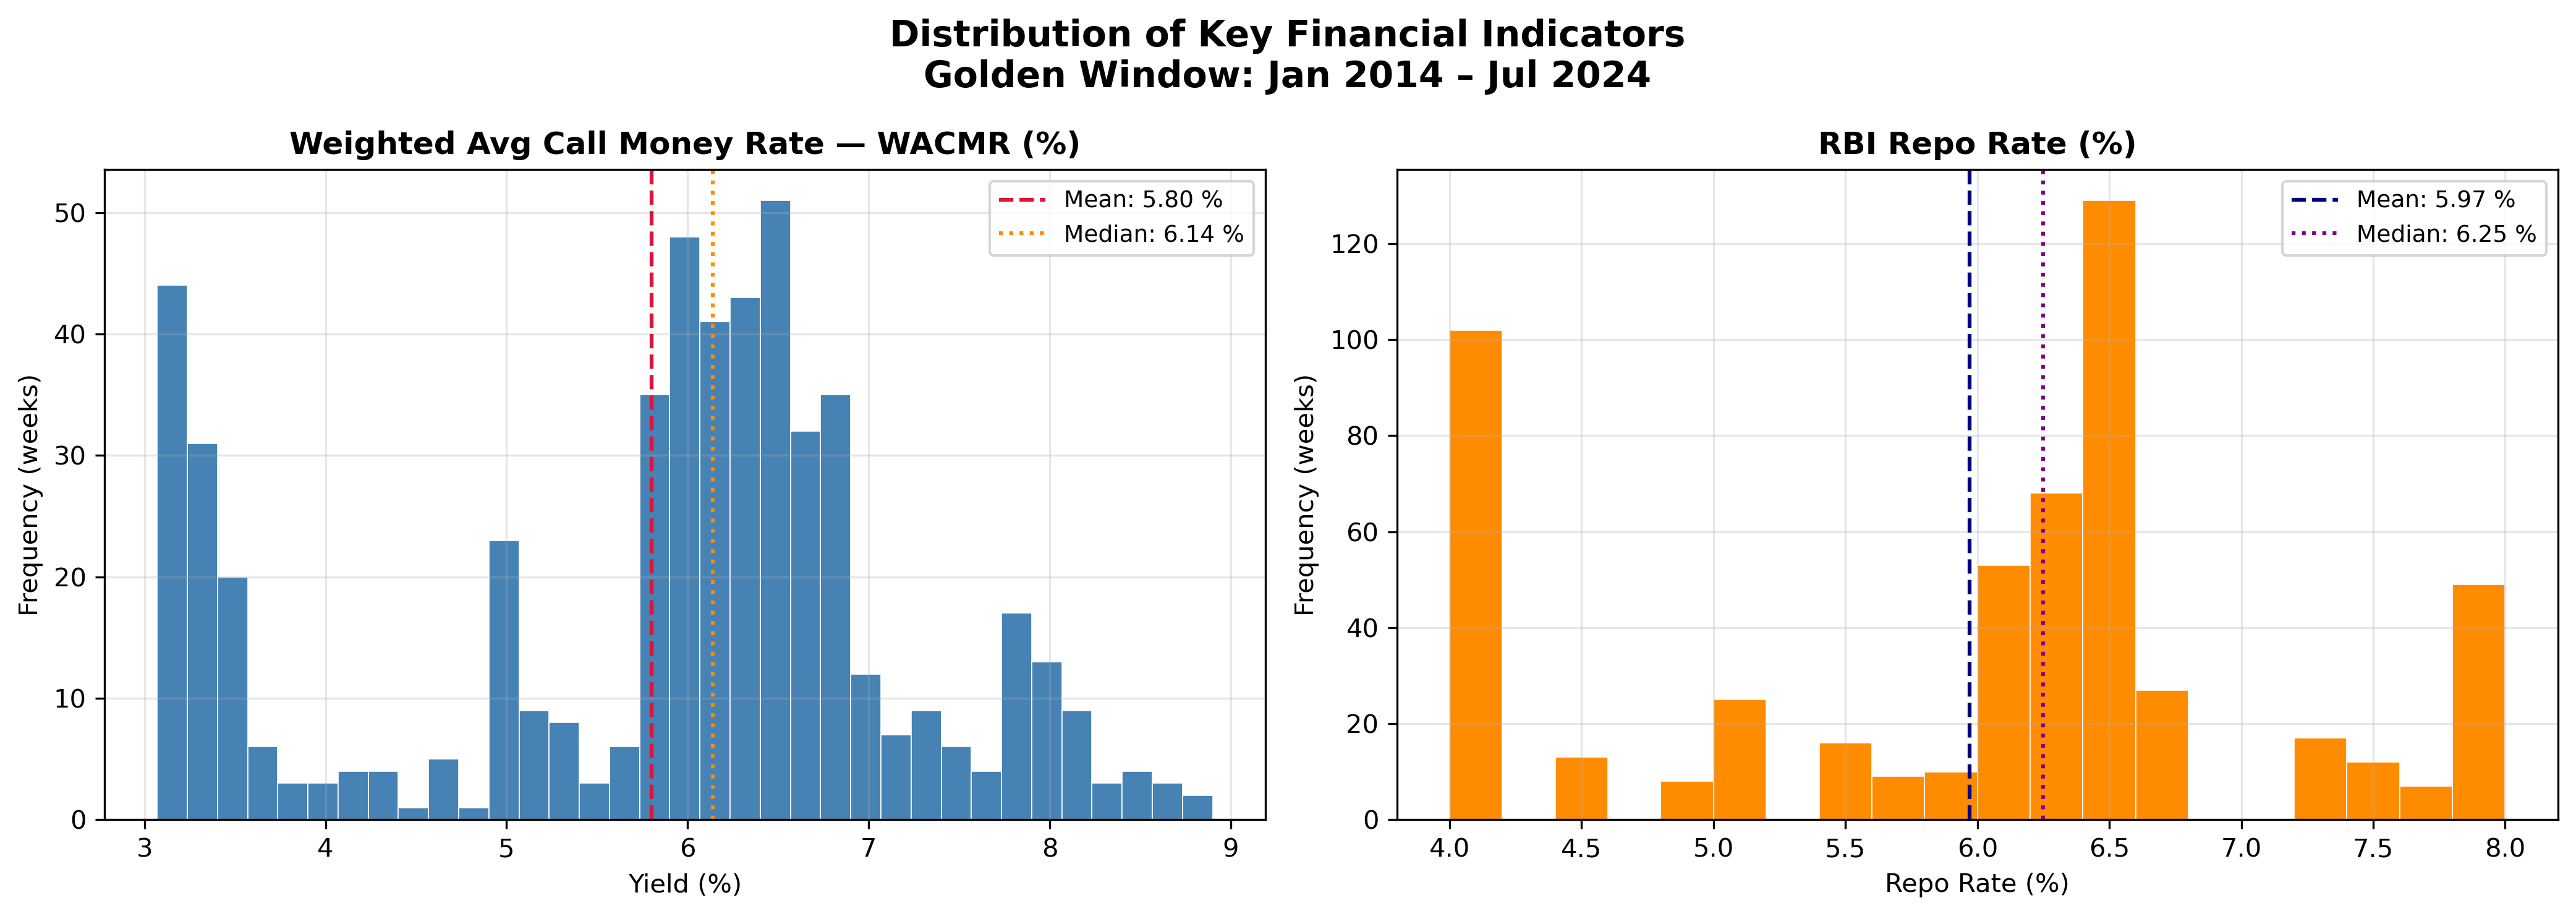
\includegraphics[width=0.92\linewidth]{../../visualizations/eda_distributions.png}
\caption{Histograms of WACMR and its principal corridor neighbours.
The bimodal WACMR shape is clearest in the top-left panel.}
\label{fig:eda-distributions}
\end{figure}

A short statistical summary anchors the qualitative impression. The
target variable is non-null for all 545 weeks, with mean 5.803\% and
standard deviation 1.462\%. The minimum (3.07\%) occurs in December
2020 at the trough of the COVID accommodation; the maximum (8.90\%)
occurs in February 2014 just after the post-taper-tantrum tightening.

\subsection{Missingness and density filtering}

A strict density rule was applied during alignment: any column with
less than 75\% non-null coverage on the Friday-aligned grid was
dropped. Of 109 raw NDAP columns, 18 were eliminated under this rule,
mostly from the older portions of the RBI balance-sheet table where
sub-categories were not reported before 2016. Two further columns
(\texttt{rates\_I7496\_28} Market Repo Rate and \texttt{rates\_I7496\_29}
Certificate of Deposit Rate) had 17.4\% missing values, marginally
below the threshold but retained for economic relevance and imputed
with the column median.

CPI was forward-filled with a maximum four-week carry, which is the
natural operational behaviour for monthly inflation indices. Yahoo
Finance OHLCV was 100\% complete after the warmup-trim step.

\begin{methodbox}
The density rule and the imputation strategy together give a panel
where every column either covers the full 545-week window or is
filled in a way that preserves the statistical signal. This was
verified by re-running the K-Means analysis with the two imputed
columns dropped; the silhouette score moved by less than 0.005, so
the imputation does not drive the regime result.
\end{methodbox}

\subsection{Anomalies and known structural events}

Three anomalies in the WACMR series are visible in
Figure~\ref{fig:target-timeseries} and have known macroeconomic
explanations.

\begin{itemize}
\item \textbf{November 2016, demonetisation.} A sharp downward spike,
  caused by the sudden injection of high-powered money as old notes
  were withdrawn and bank deposits ballooned.
\item \textbf{September--December 2018, NBFC liquidity squeeze.} A
  noticeable upward bump as overnight funding markets reacted to the
  IL\&FS default and the broader contagion.
\item \textbf{March 2020, COVID-19 emergency rate cut.} The
  largest visible discontinuity in the entire series, where the Repo
  Rate was cut by 75 bps in an out-of-cycle decision and WACMR
  followed within the week.
\end{itemize}

These anomalies are not removed from the panel, since they are real
data points. They will reappear later as the largest tail residuals
in the supervised model.

\subsection{Pairwise relationships among features}

Pearson correlation between the target and each feature was computed
on the full panel. The top correlated features are, predictably, the
corridor rates and the autoregressive lags, which together foreshadow
the SHAP results presented in Section~\ref{sec:methods}. Four notable
correlations sit outside the rate corridor.

\begin{table}[H]
\caption{Top non-corridor Pearson correlations against
\texttt{target\_wacmr}. The corridor rates Repo, Reverse Repo, and MSF
are excluded from this short table because their dominance would crowd
out the rest.}
\label{tab:correlations-noncorridor}
\renewcommand{\arraystretch}{1.2}
\rowcolors{2}{SoftGray}{white}
\begin{tabularx}{\linewidth}{@{} Y l l Y @{}}
\toprule
\rowcolor{Slate}\color{white}\textbf{Feature} &
\color{white}\textbf{Domain} &
\color{white}\textbf{Pearson $r$} &
\color{white}\textbf{Plain reading} \\
\midrule
\texttt{rates\_I7496\_27} (CBLO/Tri-party) & Debt market rates & 0.96 & Almost a clone of WACMR. \\
\texttt{rates\_I7496\_29} (CD Rate) & Debt market rates & 0.85 & Bank short-term funding cost. \\
\texttt{cp\_I7505\_*} (CP outstanding) & Commercial paper & 0.42 & Risk-on activity correlates with rates. \\
\texttt{usdinr\_intc} (Close) & Forex & $-0.18$ & Weak inverse, currency strengthens as rates fall. \\
\texttt{nifty\_intc} (Close) & Equity & $-0.27$ & Weak inverse, equities benefit from low rates. \\
\bottomrule
\end{tabularx}
\end{table}

The two market-sentiment correlations are weak in absolute terms.
This is the first quantitative hint that the equity and forex channels
will not survive a multivariate analysis once the corridor rates are
already in the feature set, a result that is confirmed by the SHAP
analysis in Section~\ref{sec:methods}.
